\section{Udsætning af vildt}

\begin{frame}
  \vspace{3em}
  \begin{center}
    {\LARGE \textbf{Udsætning af vildt}
    }
    \\
    \vspace{1em}
    Bekendtgørelse om udsætning af vildt, jagtmåder og jagtredskaber
    \\
    \vspace{1em}
    BEK nr 1652 af 19/12/2017, Kapitel 6
  \end{center}
\end{frame}

\begin{frame}{Generelt vedrørende udsætning af vildt}

\textbf{Hovedregel:} \\
Vildt må \textbf{ikke} udsættes i naturen uden tilladelse fra myndigheden.

\textbf{Undtagelse – kun disse tre arter må udsættes uden tilladelse:}
\begin{itemize}
    \item \textbf{Fasan} (Phasianus colchicus): 1. april – 31. august
    \item \textbf{Agerhøne} (Perdix perdix): 1. april – 15. august
    \item \textbf{Gråand} (Anas platyrhynchos): 1. april – 31. juli (i ferske vande)
\end{itemize}

\textbf{Vigtige fælleskrav for alle tre arter:}
\begin{itemize}
    \item \textbf{Alle} udsætninger skal indberettes digitalt senest 1 uge efter
    \item Udsætning af \textbf{mere end 100 fugle i alt} (fasan + agerhøne + gråand) kræver gennemført \textbf{godkendt kursus}
    \item Fravigelse fra basisreglerne (f.eks. højere tæthed end 1/ha for fasan/agerhøne) kræver \textbf{biotopplan}
\end{itemize}

\textbf{Alle andre vildtarter:} \\
Kræver særskilt tilladelse – udsætning er generelt forbudt.

\end{frame}




\begin{frame}{Udsætning af fasaner}

\begin{columns}[T] % T = top-aligned

\begin{column}{0.48\textwidth}
\textbf{Regler ved udsætning af fasaner:}
\begin{itemize}
    \item Kan udsættes 1. april til 31. august 
    \item Under 100ha max 100 fugle
    \item Over 100ha 1 fugl pr ha
    \item Biotopplan implementeret op til 7 fugle pr ha
    \item 5 årig biotopplan 2 år inde implementeret op til 12 fugle pr ha
    \item Afvigelser fra 1 fugle pr ha afhænger af pointsystem
    \item Alle udsætninger skal indberettes senest 1 uge efter udsætningen
\end{itemize}
\end{column}

\begin{column}{0.3\textwidth}
    % Vælg én af disse – de ser godt ud i præsentation
    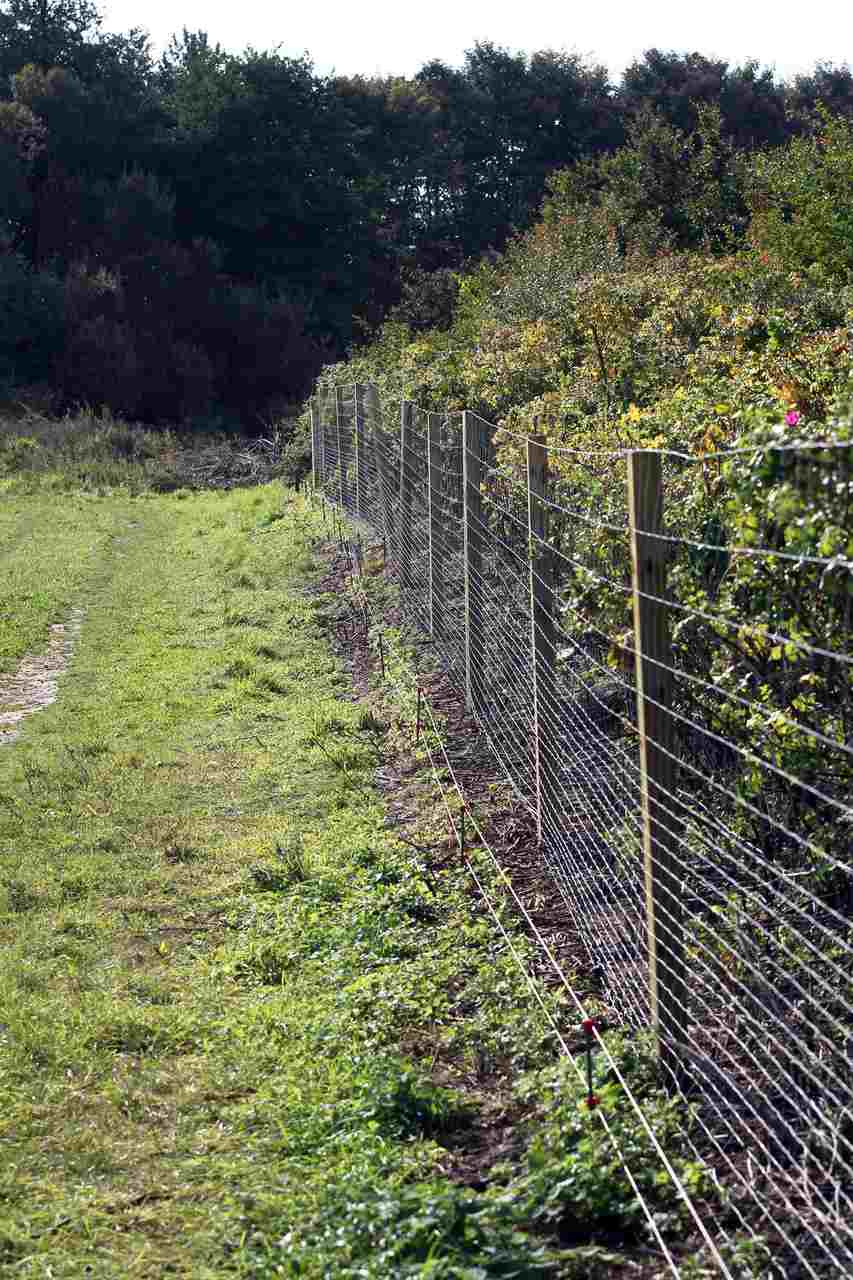
\includegraphics[width=\textwidth]{Billeder/Vildtforvaltning/udsætning/fasanvoilere.jpg}
    % Eller brug et af de gode eksempler:
    % \includegraphics[width=\textwidth]{vegetationsstriber_midtmark_ex.jpg}
\end{column}

\end{columns}

\end{frame}



\begin{frame}{Udsætning af agerhøns }

\begin{columns}[T] % T = top-aligned

\begin{column}{0.48\textwidth}
\textbf{Regler ved udsætning af agerhøns:}
\begin{itemize}
    \item Kan udsættes 1. april til 15. august
    \item Under 100 ha max 100 fugle
    \item Over 100 ha 1 fugl pr. ha
    \item Biotopplan implementeret op til 4 agerhøns pr. ha)
    \item 5-årig biotopplan 2 år inde implementeret op til max 4 agerhøns pr. ha
    \item Afvigelser fra 1 fugl pr. ha afhænger af pointsystem
    \item Alle udsætninger skal indberettes senest 1 uge efter udsætningen
\end{itemize}
\end{column}

\begin{column}{0.4\textwidth}
    % Godt billede af agerhøne eller biotop med agerhøns
    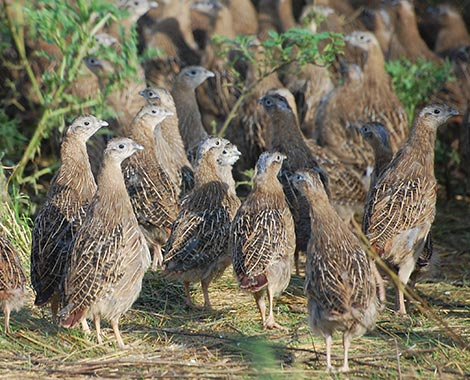
\includegraphics[width=\textwidth]{Billeder/Vildtforvaltning/udsætning/agerhøns.jpg}
    % Alternativer: agerhøne_i_mark.jpg eller vegetationsstriber_agerhoene.jpg
\end{column}

\end{columns}

\end{frame}




\begin{frame}{Udsætning af gråænder}

\begin{columns}[T] % T = top-aligned

\begin{column}{0.48\textwidth}
\textbf{Regler i ferske vande:}
\begin{itemize}
    \item Kan udsættes 1. april til 31. juli
    \item 1 ælling pr. 150 m² åben vandflade
    \item Eller 1 voksen and pr. 300 m² åben vandflade
    \item Ingen generel ha-begrænsning som ved fasan/agerhøne
    \item Ingen biotopplan-krav for højere antal
    \item Alle udsætninger skal indberettes senest 1 uge efter udsætningen
    \item Over 100 fugle (samlet med fasan/agerhøne) kræver godkendt kursus
\end{itemize}
\end{column}

\begin{column}{0.3\textwidth}
    % Vælg én af disse – de ser godt ud i præsentation
    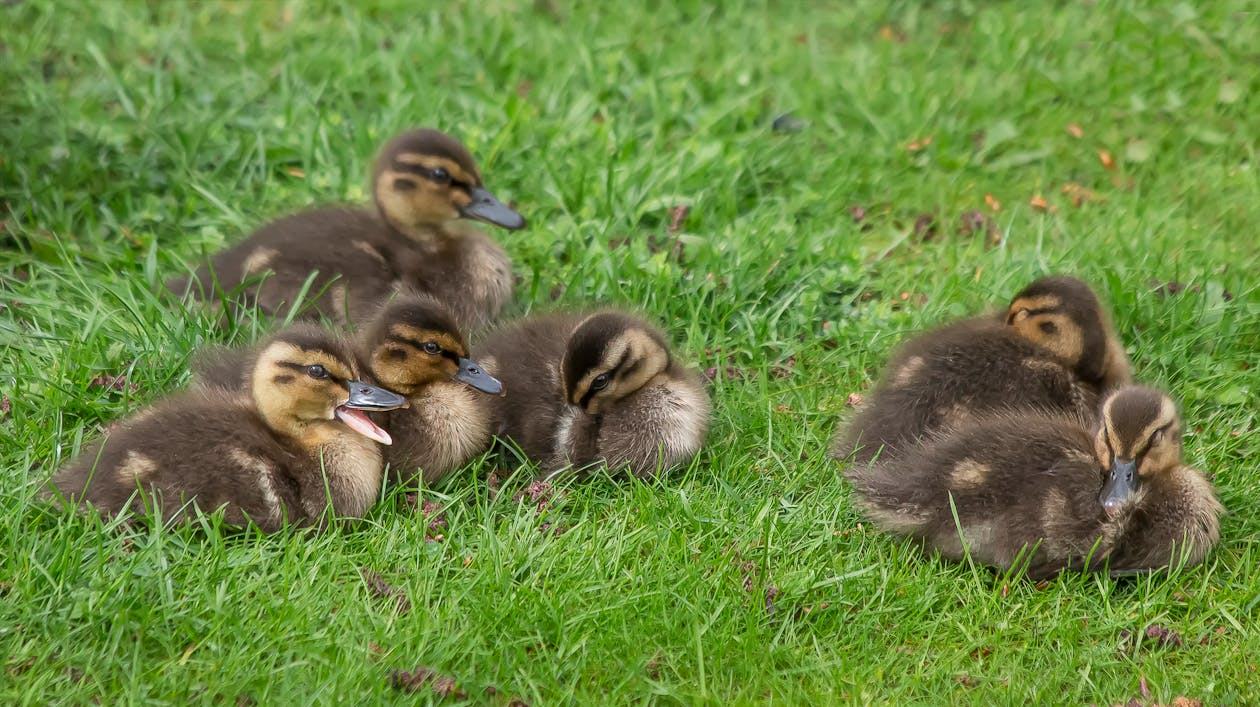
\includegraphics[width=\textwidth]{Billeder/Vildtforvaltning/udsætning/gråandeællinger.jpeg}
    % Eller brug et af de gode eksempler:
    % \includegraphics[width=\textwidth]{vegetationsstriber_midtmark_ex.jpg}
\end{column}

\end{columns}

\end{frame}